\begin{wavepdfonly}
% Shared modern PDF/EPUB cover.  The EPUB rasterizes this exact TeX cover.
% The cover artwork is The Met Open Access image DP130155 / object JP1847.
\definecolor{WaveCoverBlue}{HTML}{213E5E}
\definecolor{WaveCoverPaper}{HTML}{FBF7EC}

\newcommand{\WaveModernCover}{%
  \thispagestyle{empty}%
  \pagecolor{WaveCoverPaper}%
  \begin{center}
  \vspace*{-0.28in}
  {\color{WaveCoverBlue}\fontsize{42}{44}\selectfont\bfseries WAVE MOTIONS\par}
  \vspace{-0.05in}
  {\color{WaveCoverBlue}\fontsize{40}{43}\selectfont\bfseries IN THE OCEAN\par}
  \vspace{0.10in}
  {\color{WaveCoverBlue}\fontsize{20}{23}\selectfont\itshape Myrl's View\par}
  \vspace{0.14in}
  \setlength{\fboxrule}{0.55pt}%
  \setlength{\fboxsep}{2.5pt}%
  {\color{WaveCoverBlue}%
   \fbox{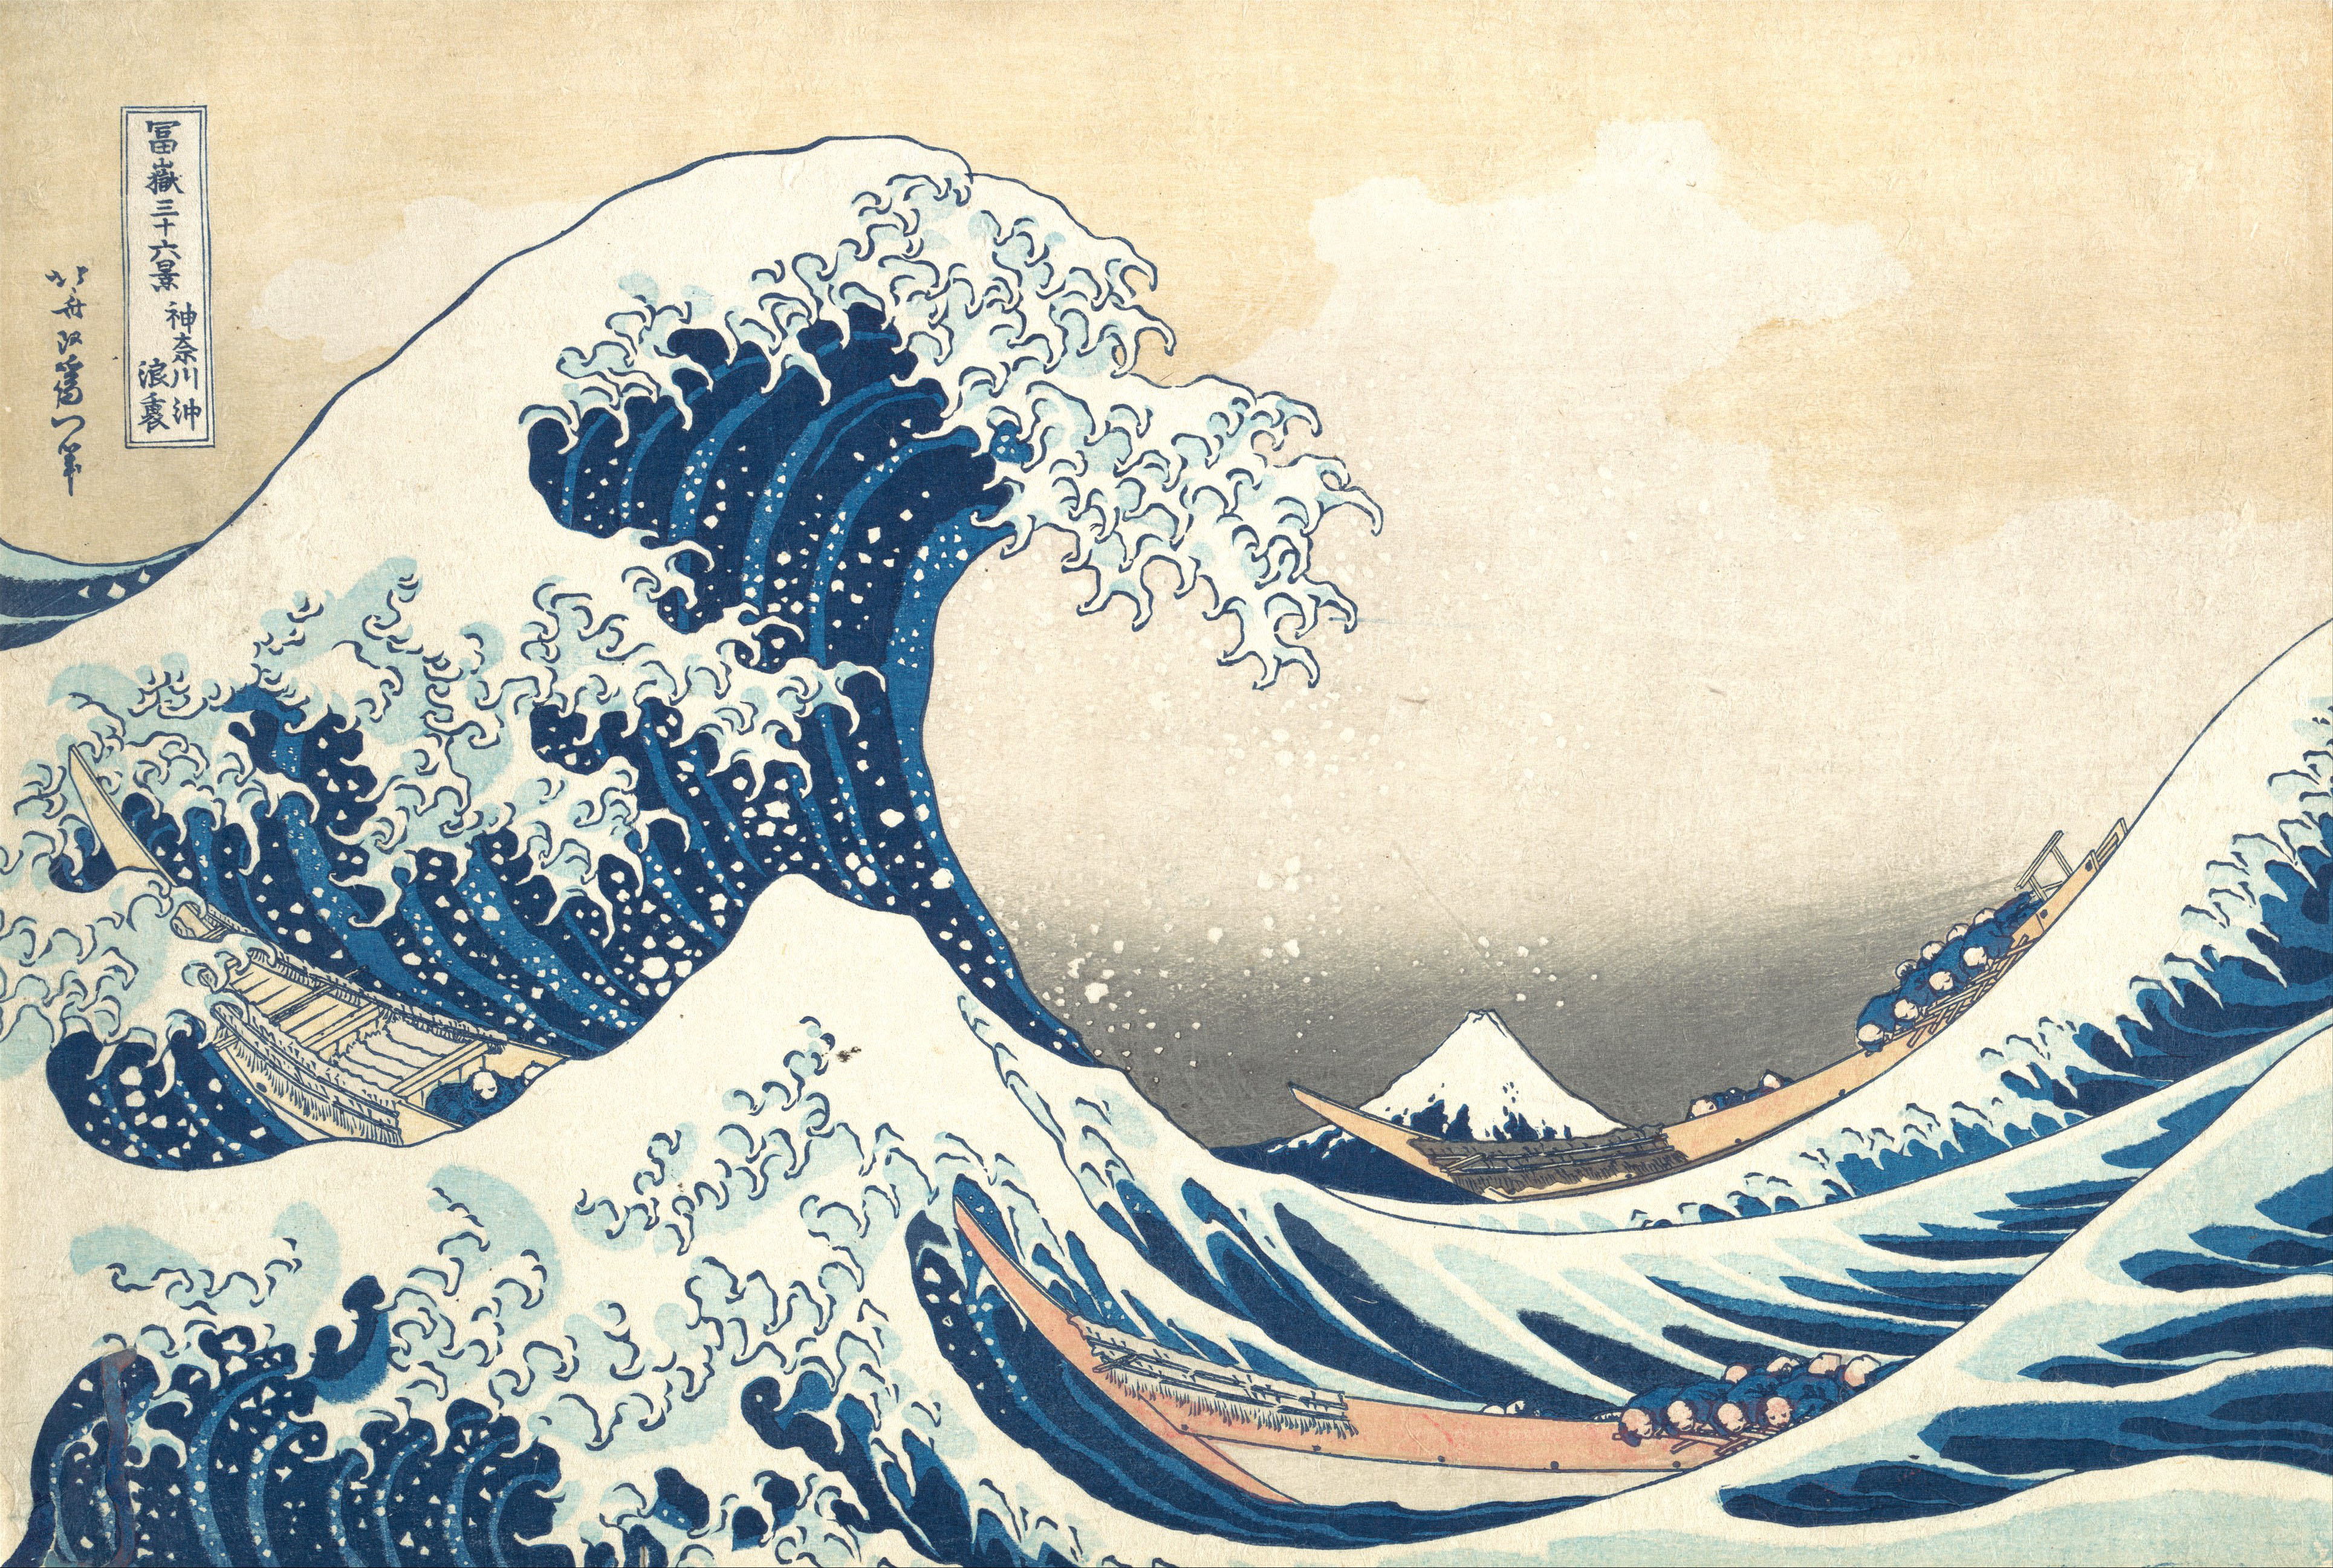
\includegraphics[width=0.965\linewidth]{figures/frontmatter/great-wave-met-dp130155.jpg}}\par}
  \vspace{0.16in}
  {\color{WaveCoverBlue}\fontsize{15}{18}\selectfont\itshape Presented to Myrl C. Hendershott\par}
  \vspace{0.13in}
  {\color{WaveCoverBlue}\fontsize{19}{22}\selectfont\bfseries David C. Chapman and\par}
  \vspace{0.01in}
  {\color{WaveCoverBlue}\fontsize{19}{22}\selectfont\bfseries Paola Malanotte-Rizzoli\par}
  \end{center}%
}

\WaveModernCover
\end{wavepdfonly}
\begin{wavewebonly}
\thispagestyle{empty}
\begin{center}
\vspace*{0.78in}
{\sffamily\color{WaveAccent}\fontsize{27}{31}\selectfont\bfseries WAVE MOTIONS IN THE OCEAN\par}
\vspace{0.22in}
{\fontsize{18}{22}\selectfont\itshape Myrl's View\par}
\vspace{0.82in}
{\large \textit{Presented to} \textbf{Myrl C. Hendershott}\par}
\vfill
{\large \textbf{David C. Chapman and Paola Malanotte-Rizzoli}\par}
\vspace{0.10in}
{\normalsize August 1989\par}
\vfill
{\small\sffamily Digital edition by \textbf{Albert M. W. Yau}\par}
\vspace{0.08in}
{\small\sffamily August 2026\par}
\end{center}
\end{wavewebonly}
\clearpage
\nopagecolor

\wavepagenumbering{roman}

\chapter*{Preface — David C. Chapman}
\addcontentsline{toc}{chapter}{Preface — David C. Chapman}
When I volunteered to teach the MIT/WHOI Joint Program core course on
``Wave Motions in the Ocean and Atmosphere'' in Spring 1989, I naturally turned for
guidance to the notes I had acquired from a similar course taken while a student at
Scripps Institution of Oceanography. In an attempt to broaden the scope of the course,
I borrowed a set of notes from Paola Malanotte-Rizzoli who taught the MIT/WHOI
core course from 1983-1985. It didn't take long to recognize that Paola's notes were
nearly identical to mine because she had also based hers on the waves course she had
taken at Scripps. In both cases, the Scripps course was taught by our former advisor
Myrl Hendershott, which means that at least two generations of Physical
Oceanography students have learned the ``Hendershott view'' of waves. Considering
the seemingly timeless nature of the concepts presented in Myrl's course as well as the
profound influence Myrl has had on Paola and myself through both his teaching and
his advising, we decided to compile these notes into a form which could be distributed
to students and, at the same time, serve as a tribute to Myrl. Thus, with the exception
of some minor modifications, additions and deletions that Paola and I have made, the
notes contained herein are those developed by Myrl for his course. We hope that these
notes will be as clear and as useful to future readers as they have been to us.

\wavesignature{David C. Chapman}{Woods Hole}{1989}

\chapter*{Preface — Paola Malanotte-Rizzoli}
\addcontentsline{toc}{chapter}{Preface — Paola Malanotte-Rizzoli}
These notes have been collected and assembled in different ways over the years
by two people successively, Paola Malanotte-Rizzoli and Dave Chapman. The present
and chronologically latest version has been put together by Dave and constitutes the
bulk of the waves course he taught in Spring 1989. When I taught the course during
the years 1983-85, the chapter on acoustic waves was absent. I had instead a section on
the Garrett and Munk spectrum and a chapter on nonlinear wave interactions. These
differences reflect the different years in which Dave and I took the waves course at
Scripps Institution of Oceanography from our former advisor Professor Myrl C.
Hendershott and the modifications that Myrl had made in his course in successive
years. Thus the inspirational source or, rather, the actual bulk of these notes is the
waves course taught by Myrl at Scripps.

Myrl Hendershott has been at W.H.O.I. this summer as Principal Lecturer of
the GFD Summer School on Ocean Circulation. This opportunity, plus Dave
Chapman's diligence and patience in typing the notes on his word processor together
with formulas and equations (the latter were handwritten in my own set of notes), has
motivated us to produce this report as an homage to Myrl. Without him, we would
both have had a much harder and more time-consuming role in putting together a
decent course on waves. More importantly, Myrl is in many ways responsible for
whatever success we have had in the field of Oceanography.

I must add here a personal note. Hearing Myrl again as a teacher this summer
after so many years, I have realized how much he has influenced my way of thinking
and teaching. On the not-so-positive side (I will not say negative):
\begin{itemize}[leftmargin=2.2em,itemsep=0.2em,topsep=0.3em]
\item like him, I ``scribble'' a lot on the blackboard.
\item like him, I erase with my left hand what I have just written with my right hand.
\item like him, I put $\ell$ ($x$ wavenumber) before $k$ ($y$ wavenumber)
\end{itemize}
As the letters $j,k,x,y,w$ do not exist in the Italian alphabet, $k$ coming before or after
$\ell$ was supremely unimportant to me. On the positive side, Myrl was absolutely the
best teacher I had in the various courses I took at Scripps. His lectures were always
interesting, imaginative and full of physical insight. Looking back, I realize that a
great deal of the important oceanographic concepts and ideas I learned over the years
go back to my long association with Myrl as teacher, advisor, colleague and, last but
not least, dear friend. I hope I absorbed from him some of the positive qualities too.

\wavesignature{Paola Malanotte-Rizzoli}{Woods Hole}{1989}

\clearpage

\chapter*{Editor's note}
\addcontentsline{toc}{chapter}{Editor's note}

These lecture notes have been preserved on James Pringle's website and have
recently been reconstructed in \LaTeX. This digital edition has been
authorized by Paola Malanotte-Rizzoli for release under the Creative Commons
Attribution--NonCommercial--ShareAlike 4.0 International license
(CC BY-NC-SA 4.0).

The reconstruction is a work in progress, with assistance from OpenAI's GPT-5.6 Sol.

\wavesignature{Albert M. W. Yau}{Stony Brook}{2026}

% Keep the historical photograph with the Editor's note. The non-floating H
% placement guarantees that the cover credit which follows is the final item on
% this page rather than being separated from the photograph by float movement.
\begin{figure}[H]
  \centering
  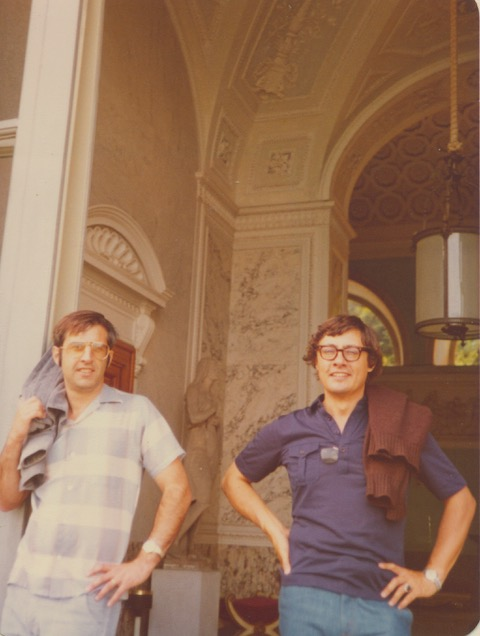
\includegraphics[width=0.82\linewidth]{figures/frontmatter/salmon-hendershott-como-1980.jpeg}
  \par\smallskip
  {\small Rick Salmon (left) and Myrl Hendershott at Villa Carlotta, Lake Como,
  during the International School of Physics ``Enrico Fermi,'' Course LXXX,
  \textit{Topics in Ocean Physics}, July 1980.\par}
\end{figure}

\wavecovercredit

\clearpage

\tableofcontents
\clearpage
